\documentclass[12pt]{report}
\usepackage[french]{babel}
\usepackage[utf8]{inputenc}
\usepackage[T1]{fontenc}
\usepackage[top=2cm, bottom=2cm, left=2cm, right=2cm]{geometry}
\usepackage{graphicx}
\usepackage{xcolor}
\usepackage{float}
\usepackage[french, onelanguage, boxruled, longend]{algorithm2e}
\usepackage{setspace}
\usepackage{multirow}
\usepackage{minted}
\usepackage{tikz}
\usepackage{amsmath}
\usepackage{amsfonts}

\newcommand{\HRule}{\rule{\linewidth}{0.5mm}}

\begin{document}
    \begin{titlepage}
        \begin{center}
            \textbf{République Algérienne Démocratique et Populaire}\\
            \textbf{Ministère de l'Enseignement Supérieur et de la Recherche Scientifique}\\[1cm]
            
            
\includegraphics[scale=0.5]{./ressources/USTHB_Logo.png}\\[1cm]
            
            \large
            \textbf{Université des Sciences et de la Technologie Houari Boumédiène}\\[0.5cm]
            \textbf{Faculté d'Electronique et d'Informatique}\\
            \textbf{Département Informatique}\\[0.5cm]

            \Large
            \textbf{Master Systèmes Informatiques intelligents}\\[0.5cm]
            
            \textbf{Module :} Conception et Complexité des Algorithmes

            \HRule \\[0.4cm]
            \LARGE{\textbf{Rapport de projet 2 de TP}\\
            \textit{}\\[0.4cm]}
            \HRule \\[2cm]
            
            \large
            \textbf{Réalisé par :}\\
            AIT AMARA Mohamed, 181831072170\\
            BOUROUINA Rania, 181831052716\\
            CHIBANE Ilies, 181831072041\\
            HAMMAL Ayoub, 181831048403
            
            \vfill
            Année universitaire : 2021 / 2022
        \end{center}
    \end{titlepage}
    \normalsize

    \tableofcontents

    \newpage
    \onehalfspacing
    \chapter{la Tour de Hanoi, historique et présentation du problème}

\section{Introduction Historique}
La Tour de Hanoi est inspirée à Lucas par l’un de ses amis, le professeur Claus de Siam qui raconte une histoire ayant lieu au coeur du temple Kashi Vishwanath :
Trois aiguilles de diamant, plantées dans une dalle d’airain. […] Sur une de ces aiguilles, Dieu enfila au commencement des siècles, 64 disques d’or pur, le plus large reposant sur l’airain, et les autres, de plus en plus étroits, superposés jusqu’au sommet.

C’est la tour sacrée du Brahmâ. Nuit et jour, les prêtres se succèdent sur les marches de l’autel, occupés à transporter la tour de la première aiguille sur la troisième, sans s’écarter des règles fixes que nous venons d’indiquer, et qui ont été imposées par Brahma. Quand tout sera fini, la tour et les brahmes tomberont, et ce sera la fin des mondes !

Edouard Lucas, Récréations mathématiques, tome 3, (1892), réédité par la Librairie Albert Blanchard, (1979), p. 58
\subsection{fait amusant}
Comme indiqué ci-dessous, un jeu à 64 disques requiert un minimum de 264-1 déplacements (soit 18 446 744 073 709 551 615 déplacements). En admettant qu'il faille 1 seconde pour déplacer un disque, ce qui fait 86 400 déplacements par jour, la fin du jeu aurait lieu au bout d'environ 213 000 milliards de jours, ce qui équivaut à peu près à 584,5 milliards d'années, soit 43 fois l'âge estimé de l'univers (13,7 milliards d'années selon certaines sources)

\section{Présentation du problème}
Les tours de Hanoï (originellement, la tour d'Hanoïa) sont un jeu de réflexion imaginé par le mathématicien français Édouard Lucas, et consistant à déplacer des disques de diamètres différents d'une tour de « départ » à une tour d'« arrivée » en passant par une tour « intermédiaire », et ceci en un minimum de coups, tout en respectant les règles suivantes :

->on ne peut déplacer plus d'un disque à la fois.
->on ne peut placer un disque que sur un autre disque plus grand que lui ou sur un emplacement vide.

\begin{figure}[H]
    \centering
        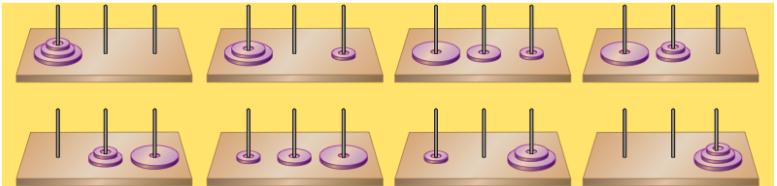
\includegraphics[scale=0.5]{./ressources/Présentation_du_problème.png}
        \caption{Exemple d'une solution dans le cas de trois disques}
    \label{fig:representationProbleme}
\end{figure}

\subsection{Polémique}
Il existe toujours cette confusion dans certains articles scientifiques qui mentionnent que le problème de la tour de Hanoi est NP alors que ce n'est pas le cas.

Dans ce problème les étapes correctes peuvent être déterminées dès le départ sans avoir besoin d'une recherche d'essais-erreurs pour prendre la bonne décision. Par conséquent, ce problème n'est pas un problème de décision, auquel des classes telles que NP s'appliquent.

C'est plus un problème de fonction. La complexité temporelle est en effet déterminée par le nombre d'étapes à sortir, qui est de 2n-1, c'est-à-dire $O(2^n).$
La classe correspondante serait donc FEXPTIME-Complete, le préfixe F signifiant Function, et Complete signifiant que cela ne peut se faire en un temps inférieur à exponentiel (comme P). Elle est analogue à la classe EXPTIME-Complete pour les problèmes de décision, c'est-à-dire $O(2^{polynomial(n)})$.

Il faut savoir que la classe EXPTIME En théorie de la complexité, est la classe de complexité qui est l'ensemble des problèmes de décision décidés par une machine de Turing déterministe en temps exponentiel.  Mais il existe des classes plus grosses comme EXPSPACE et NEXPTIME (respectivement les problèmes pouvant être résolus en espace exponentiel, et en temps exponentiel sur machine non déterministe).
L'illustration ci-dessous montre le diagramme d'inclusions des classes de complexité classiques :
\begin{figure}[H]
    \centering
        \includegraphics[scale=0.5]{./ressources/Les_classes_de_complexité.png}
        \caption{Diagramme d'inclusions des classes de complexité classiques.}
    \label{fig:classeComplexite}
\end{figure}

\subsection{Définition formelle du problème}
Il est facile de démontrer par récurrence que si n est le nombre de disques, il faut 2n - 1 coups au minimum pour parvenir à ses finsc, quantité qui augmente très rapidement avec n. En effet, soient A, B et C les trois emplacements des tours ; notons $x_n$ le nombre de déplacements de disques nécessaires au déplacement d'une tour complète. Pour déplacer une tour de n disques de A vers C, on effectue ces trois étapes :

déplacer la tour des n-1 premiers disques de A vers B (étape qui nécessite $x_{n-1}$ déplacements, d’où la récurrence) ;
déplacer le plus grand disque de A vers C (un déplacement supplémentaire) ;
déplacer la tour des n-1 premiers disques de B vers C (à nouveau $x_{n-1}$ déplacements).
Le nombre de déplacements de disques vérifie donc la relation de récurrence :

\hspace*{6.4cm}                        $x_0 = 0$ \\
\hspace*{7cm}                        $x_n = 2x_{n-1}+1$ si $n >= 1$ \\
ce qui donne bien : \\
\hspace*{7cm}                        $x_n = 2^n - 1$ \\

On peut montrer que la méthode décrite ici donne la séquence optimale (celle qui nécessite le moins de coups), et que celle-ci est unique. En effet, pour déplacer la tour de n disques de A vers C, on devra forcément, à un moment ou à un autre, déplacer le plus grand disque de A vers C, et pour ce faire, on devra avoir empilé les n-1 premiers disques en B.

\section{Conclusion}
Dans ce chapitre on a parlé de l'origine du problème de la tour de hanoi et on l'a expliqué  d'une manière classique et générale. Dans ce qui suit, on présentra notre solution récursive ainsi que des exemples démonstratifs. 


    \newpage
    \onehalfspacing
    \chapter{Présentation du la solution}

\section{Modélisation de la solution}
Dans ce problème, chaque anneau porte un numéro séquentiel unique $a_i \in [1, n]$ qui représente sa taille tel que $n$ est le nombre maximal d'anneaux (E.g. l'anneau avec le nombre $1$ est plus petit que l'anneau avec le nombre $3$).
\par
De plus, on modélise chaque tour par un tableau $T_j$ d'une taille égale au nombre maximum d'anneaux $n$. Si un niveau $i$ de la tour $j$ contient un anneau $a_{i'}$, alors $T[j, i] = a_{i'}$, sinon $T[j, i] = 0$. Le niveau le plus bas de la tour (la base de la tour) est placé à la dernière case du tableau ; $\forall j$ $T[j, n]$ est le niveau le plus bas de la tour (voir Figure \ref{fig:rep_tour}).

\begin{figure}[h!]
    \begin{center}
        \begin{tikzpicture}
            \draw (0,0) rectangle (2,5);
            \draw (0,1) -- (2,1);
            \draw (0,4) -- (2,4);
            \draw [dashed] (0,2) -- (2,2);
            \draw [dashed] (0,3) -- (2,3);
            %\node at (1,2.5) {- - -};

            \node [left] at (-1,0.5) {T[j, n]};
            \node at (1,0.5) {n};
            \node [right] at (3,0.5) {l'anneau le plus grand};

            \node [left] at (-1,4.5) {T[j, 1]};
            \node at (1,4.5) {1};
            \node [right] at (3,4.5) {l'anneau le plus petit};

            \node [below] at (1,-0.5) {T[j]};

        \end{tikzpicture}
        \caption{Exemple d'une tour avec tous les anneaux}
        \label{fig:rep_tour}
    \end{center}
\end{figure}

\par
Par conséquent, le bord de jeu peut être représenté par une matrice, colonne par colonne, où chaque colonne est en réalité une tour du jeu.

$$
\mathbf{bord} = 
\begin{pmatrix}
    T[1, 1] & T[2, 1] & ... \\
    ... \\
    T[1, n] & T[2, n] & ...
\end{pmatrix}$$

Un exemple d'initialisation classique de trois tours avec trois anneaux placés sur la première tour :

$$
\mathbf{bord} = 
\begin{pmatrix}
    1 & 0 & 0 \\
    2 & 0 & 0 \\
    3 & 0 & 0 
\end{pmatrix}
$$

\paragraph{Règles de changement d'état}
Pour passer d'un état de bord vers le suivant, on ne peut bouger qu'un seul anneau du haut d'une tour vers une autre tour, à condition que l'anneau supérieur de la tour destination ait un nombre supérieur à l'anneau qu'on veut bouger.
\par
Plus formellement, on peut déplacer le premier élément non nul d'une colonne s'il existe vers une autre colonne, s'il y a encore de la place et que le premier element non nul de la colonne destination est supérieur à celui qu'on déplace.

\section{Algorithme de résolution}
Cet algorithme récursif permet de produire la séquence exacte d'actions pour résoudre le problème des tours de Hanoi.
\par
On commence d'abord par déplacer les $n - 1$ disques de la tour de départ vers la tour intermédiaire par un appel récursif. Puis, le plus grand disque restant est transporté vers la tour d'arrivée. Ensuite, les $n - 1$ disques qui se trouvaient sur la tour intermédiaire sont déplacés vers la tour d'arrivée par le même processus récursif.

\begin{algorithm}[H]
    \SetAlgoLined
    \KwData{bord : matrice [1, 3][1, n] d'entiers, depart, arrivee, intermediaire : 1..3, nbdisques : entier}
    \KwResult{bord : matrice [1, 3][1, n] d'entiers}
    \Begin{
        \uIf{$nbdisques = 1$}{
            \tcp{S'il reste un seul disque à déplacer, on le déplace directement}
            deplacer(board, depart, arrivee)
        }\Else{
            Hanoi(bord, depart, intermediaire, arrivee, nbdisques - 1)\;
            deplacer(board, depart, arrivee)\tcp*{Deplacer le disque supérieur de la tour depart vers la tour arrivee}
            Hanoi(bord, intermediaire, arrivee, depart, nbdisques - 1)\;
        }
    }
    \caption{Hanoi}
\end{algorithm}

La fonction \emph{deplacer} permet de déplacer le disque de niveau supérieur d'une tour vers un autre.

\begin{function}[H]
    \textbf{Variable :}\\
    i, j : entier\;
    \Begin{
        \tcp{Trouver le disque supérieur de la tour depart}
        $i \leftarrow 1$\;
        \While{$i \leq n$ et $bord[depart][i] = 0$}{
            $i \leftarrow i + 1$\;
        }
        \tcp{Trouver le disque supérieur de la tour arrivee}
        $j \leftarrow 1$\;
        \While{$j \leq n$ et $bord[arrivee][j] = 0$}{
            $j \leftarrow j + 1$\;
        }
        $bord[arrivee][j - 1] \leftarrow bord[depart][i]$\;
        $bord[depart][i] \leftarrow 0$\;
    }
    \caption{deplacer(Entrée/sortie : bord : matrice {[1, 3]}{[1, n]} d'entiers, Entrée : depart, arrivee : 1..3)}
\end{function}

\paragraph{Calcul de la complexité}
La complexité est exprimée en matière de nombre d'opérations de déplacement effectuées. En l'occurrence, le nombre de déplacements est exprimé selon la suite numérique suivante :
$$ h(1) = 1 $$
$$ h(n) = 2 * h(n - 1) + 1 $$
où $n$ représente le nombre total de disque à déplacer.

En remplaçant $h(n - 1)$ par la formule réccurente, on obtient :
$$ h(n) = 2 * (2 * h(n - 2) + 1) + 1 $$
$$ h(n) = 2 * (2 * (2 * h(n - 3) + 1) + 1) + 1 $$
$$ ... $$
$$ h(n) = 2^{n} - 1 $$

Ce résultat peut être démontré par récurrence comme suit :\\
Cas de base ou pour $n = 1$ :
$$ h(1) = 2^{1} - 1 = 1$$
Donc la formule est correcte pour $n = 1$.\\
Supposons que la proposition $h(i) = 2^{i} - 1$ est correcte pour $\forall i \leq n$. Montrons qu'elle est aussi correcte pour $n + 1$ :
$$ h(n + 1) = 2 * h(n) + 1$$
D'après l'hypothèse :
$$ h(n + 1) = 2 * (2^{n} - 1) + 1 $$
$$ h(n + 1) = 2^{n + 1} - 1$$
Donc la proprosition est correct $\forall n \in \mathbb{N}$.\par
Et ainsi la complexité est égale à $\mathcal{O}(2^{n})$.

\section{Algorithme de vérification}
Le problème des tours de Hanoi à trois tours admet une unique solution, sous forme d'une suite de déplacements qui génèrent un séquencement d'états intermédiaires.
\par
Pour vérifier la validité d'une solution quelconque, nous devons nous assurer que chaque déplacement est bien réglementaire (concerne le disque le plus haut et ne pose pas un disque sur un autre disque de taille plus petite) et que le dernier état engendré correspond effectivement à l'état but, c.à.d. que toutes les tours sont vides sauf la tour cible. De plus, la séquence de déplacement doit être exactement de longueur $2^{n} - 1$ tel que $n$ représente le nombre de disques, car la solution est unique, donc égale à la solution calculée par l'algorithme exact.
\par
Nous nous assurons que l'algorithme de génération de solutions produit des séquences de déplacements qui respectent ces conditions susmentionnées. Par conséquent, nous devons vérifier que le dernier état qui doit correspondre à l'état but dans lequel les anneaux sont alignés sur la tour cible ou destination.

\begin{function}[H]
    \textbf{Variable :}\\
    \Begin{
        \For{$i \leftarrow 1$ \KwTo $n$}{
            \If{$bord[arrivee][i] \neq i$}{
                \KwRet{faux}\;
            }
        }
        \KwRet{vrai}\;
    }
    \caption{verification(Entrée : bord : matrice {[1, 3]}{[1, n]} d'entiers, arrivee : 1..3) : booleén}
\end{function}

\paragraph{Calcul de complexité}
La complexité de l'algorithme de vérification est triviale, elle est égale à la complexité du parcours séquentiel des éléments d'un tableau (la tour d'arrivée).
\par
La complexité temporelle est égale à $\mathcal{O}(n)$ tel que $n$ est le nombre de disques.
\par
Quant à la complexité spatiale, sachant que la fonction de vérification ne prend que le dernier état comme paramètre, elle est donc égale à la taille de la matrice d'entiers : $3 * n * n \cong \mathcal{O}(n^{2})$.

\section{Illustration d'une instance du problème}
Nous étudions dans ce qui suit une instance du problème des tours de Hanoi avec une disposition de trois tours et trois disques sur la tour initiale.
$$
\mathbf{bord} = 
\begin{pmatrix}
    1 & 0 & 0 \\
    2 & 0 & 0 \\
    3 & 0 & 0 
\end{pmatrix}
$$
\par
L'unique solution à cette disposition est la séquence suivante de 7 déplacements :
\begin{itemize}
    \item On déplace le disque de taille 1 de la tour 1 vers la tour 3.
        $$
        \mathbf{bord} = 
        \begin{pmatrix}
            0 & 0 & 0 \\
            2 & 0 & 0 \\
            3 & 0 & 1 
        \end{pmatrix}
        $$
    \item On déplace le disque de taille 2 de la tour 1 vers la tour 2.
        $$
        \mathbf{bord} = 
        \begin{pmatrix}
            0 & 0 & 0 \\
            0 & 0 & 0 \\
            3 & 2 & 1 
        \end{pmatrix}
        $$
    \item On déplace le disque de taille 1 de la tour 3 vers la tour 2.
        $$
        \mathbf{bord} = 
        \begin{pmatrix}
            0 & 0 & 0 \\
            0 & 1 & 0 \\
            3 & 2 & 0 
        \end{pmatrix}
        $$
    \item On déplace le disque de taille 3 de la tour 1 vers la tour 3.
        $$
        \mathbf{bord} = 
        \begin{pmatrix}
            0 & 0 & 0 \\
            0 & 1 & 0 \\
            0 & 2 & 3 
        \end{pmatrix}
        $$
    \item On déplace le disque de taille 1 de la tour 2 vers la tour 1.
        $$
        \mathbf{bord} = 
        \begin{pmatrix}
            0 & 0 & 0 \\
            0 & 0 & 0 \\
            1 & 2 & 3 
        \end{pmatrix}
        $$
    \item On déplace le disque de taille 2 de la tour 2 vers la tour 3.
        $$
        \mathbf{bord} = 
        \begin{pmatrix}
            0 & 0 & 0 \\
            0 & 0 & 2 \\
            1 & 0 & 3 
        \end{pmatrix}
        $$
    \item On déplace le disque de taille 1 de la tour 1 vers la tour 3.
        $$
        \mathbf{bord} = 
        \begin{pmatrix}
            0 & 0 & 1 \\
            0 & 0 & 2 \\
            0 & 0 & 3 
        \end{pmatrix}
        $$
\end{itemize}


    \newpage
    \onehalfspacing
    \chapter{Étude expérimentale}

\section{Complexité théorique de l'algorithme de résolution}
\paragraph{Complexité temporelle}
La complexité de l'algorithme de résolution comme calculée précédemment est de l'ordre de $\mathcal{O}(2^{n})$, et elle est précisément égale à $2^{n} - 1$ qui est une complexité exponentielle.
\par
Le tableau suivant représente les temps d'exécution théorique en nanoseconde de l'algorithme de résolution selon la variation de la taille du problème (le nombre de disques) :

\small
\begin{center}
    \resizebox{\textwidth}{!}{
        \begin{tabular}{| c | c | c | c | c | c | c | c | c | c | c | c | c |}
            \hline
            N & 1 & 10 & 50 & 100 & 150 & 250 & 500 & 750 & 1000\\
            \hline
            t(ns) & 2 & 1024 & 1,1259E+15 & 1,26765E+30 & 1,42725E+4 & 1,80925E+75 & 3,27339E+150 & 5,92239E+225 & 1,07151E+301\\
            \hline
        \end{tabular}
    }
\end{center}

La figure suivante (voir Figure \ref{fig:temps_exec_th_algo_reso}) représente l'évolution du temps d'exécution théorique selon le nombre de disques :

\begin{figure}[H]
    \centering
        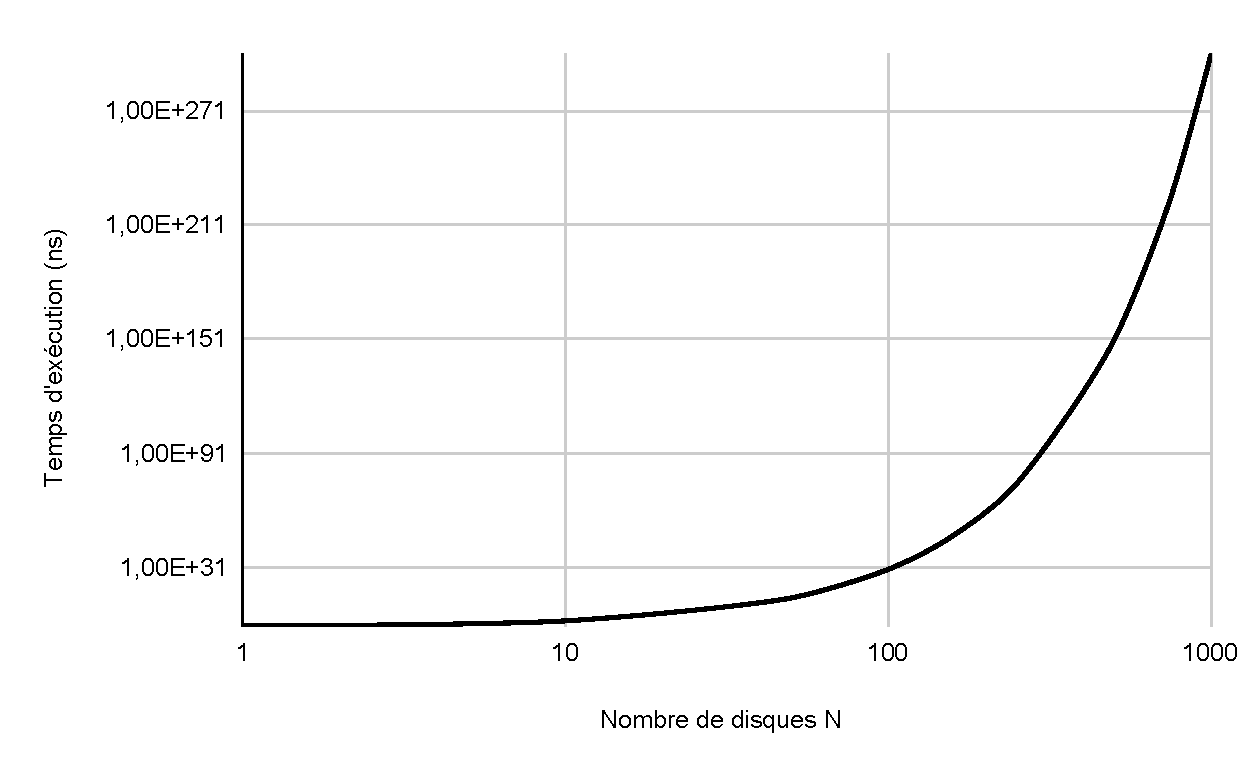
\includegraphics[scale=0.6]{./ressources/temps_execution_th_algo_reso.pdf}
        \caption{Temps d'exécution théorique de l'algorithme de résolution}
    \label{fig:temps_exec_th_algo_reso}
\end{figure} 

Depuis le graphe, nous observons que le temps d'exécution évolue de manière exponentielle selon le nombre de disques de départ. Il atteint rapidement des temps d'exécution incommensurables le rendant inexploitable.

\paragraph{Complexité spatiale}
L'algorithme exploite une matrice $3 x n$ tel que $n$ est le nombre de disques. Chaque disque est représenté par un entier de taille $4$ octets. De plus, la taille de la représentation est statique au cours de l'exécution. Par conséquent, la complexité spatiale est égale à $4 * 3 * n$ octets donc de l'ordre de $\mathcal{O}(n)$.
\par
Cependant, l'algorithme récursif fait au maximum $n$ appels récursifs (le nombre maximum d'appels est le nombre maximum de disques pouvant être déplacés à la fois). L'adresse de retour étant stockée sur $8$ octets, la taille maximale de la pile d'appel de fonctions exploitée est donc égale à $8 * n$ octets qui est de l'ordre de $\mathcal{O}(n)$.
\par
La complexité spatiale totale est donc de l'ordre de $\mathcal{O}(n)$.

\section{Complexité théorique de l'algorithme de vérification}
\paragraph{Complexité temporelle}
La complexité temporelle de l'algorithme de vérification est linéaire et elle est égale à $n \cong \mathcal{O}(n)$, car l'algorithme parcourt la tour d'arrivée et vérifie si les disques sont bien rangés dans le bon ordre.
\par
Le tableau suivant représente les temps d'exécution théorique en nanoseconde de l'algorithme de vérification selon la variation de la taille du problème (le nombre de disques) :

\small
\begin{center}
    \begin{tabular}{| c | c | c | c | c | c | c | c | c | c | c | c | c |}
        \hline
        N & 1 & 10 & 50 & 100 & 150 & 250 & 500 & 750 & 1000\\
        \hline
        t(ns) & 1 & 10 & 50 & 100 & 150 & 250 & 500 & 750 & 1000\\
        \hline
    \end{tabular}
\end{center}

La figure suivante (voir Figure \ref{fig:temps_exec_th_algo_verification}) représente l'évolution du temps d'exécution théorique selon le nombre de disques :

\begin{figure}[H]
    \centering
        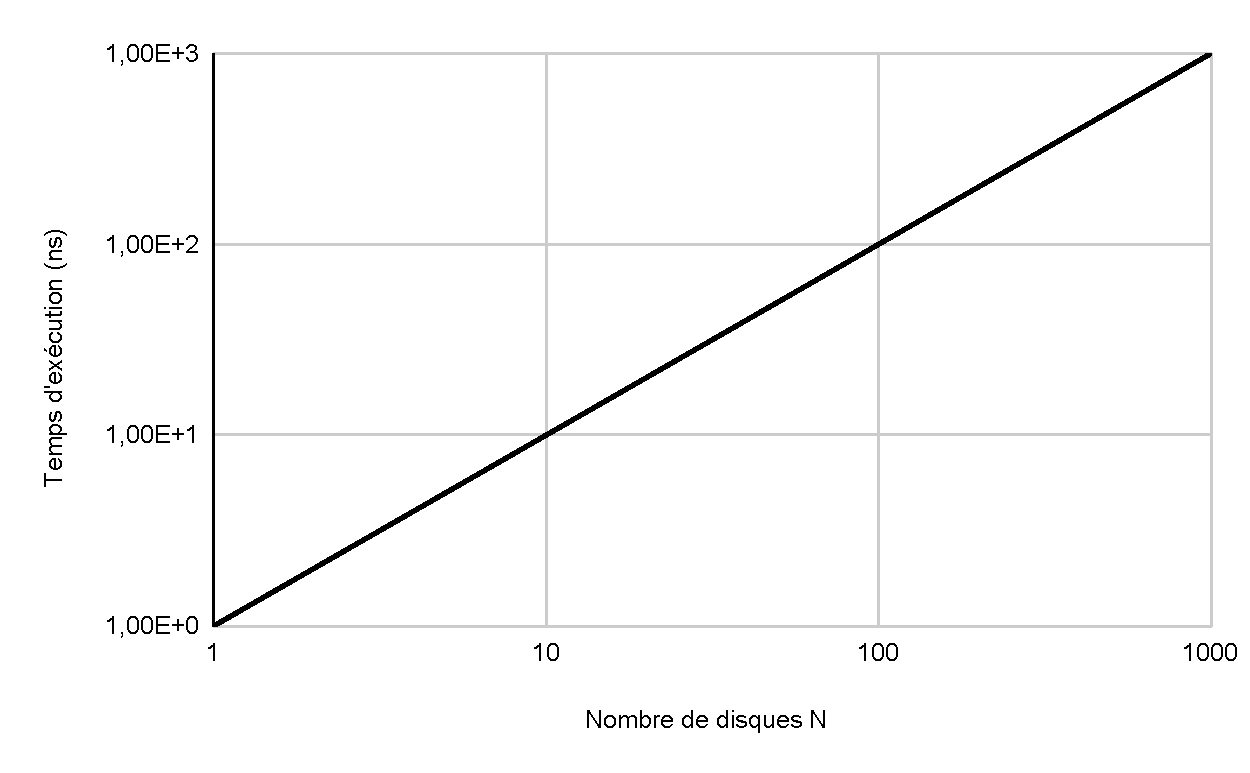
\includegraphics[scale=0.6]{./ressources/temps_execution_th_algo_verification.pdf}
        \caption{Temps d'exécution théorique de l'algorithme de vérification}
    \label{fig:temps_exec_th_algo_verification}
\end{figure} 

Depuis le graphe, nous observons que le temps d'exécution évolue avec une tendance linéaire avec l'augmentation du nombre de disques.

\paragraph{Complexité spatiale}
La complexité spatiale de l'algorithme de vérification est égale à la taille de la matrice plus l'indice de la tour cible qui est un entier, c.à.d. $3 * n + 4$ octets donc de l'ordre $\mathcal{O}(n)$.


\section{Expérimentation}

\subsection{Algorithme de résolution}

Le tableau suivant représente les temps d'exécution en nanoseconde de l'algorithme de résolution récursif selon la variation du nombre de disques.\\
\small
\begin{center}
    \begin{tabular}{| c | c | c | c | c | c | c | c |}
        \hline
        N & 3 & 5 & 7 & 10 & 15 & 20 & 25\\
        \hline
        t1(ns) & 663 & 2029 & 7829 & 59701 & 2168020 & 90192200 & 3190280000\\
        \hline
        t2(ns) & 595 & 2099 & 8018 & 60986 & 2648340 & 88261800 & 3188540000\\
        \hline
        t3(ns) & 642 & 2118 & 11230 & 62336 & 2206080 & 89520400 & 3176230000\\
        \hline
        t4(ns) & 597 & 2085 & 8118 & 61247 & 2211980 & 89318100 & 3179730000\\
        \hline
        t5(ns) & 596 & 2021 & 7724 & 61253 & 2168540 & 88693300 & 3187330000\\
        \hline
        t6(ns) & 882 & 2042 & 8044 & 61308 & 2275150 & 88450100 & 3175950000\\
        \hline
        t7(ns) & 867 & 2067 & 7977 & 63335 & 2258050 & 88788800 & 3181730000\\
        \hline
        t8(ns) & 615 & 2059 & 8085 & 63063 & 2301650 & 88529200 & 3178430000\\
        \hline
        t9(ns) & 593 & 2077 & 7942 & 60909 & 2211830 & 88074100 & 3176490000\\
        \hline
        t10(ns) & 619 & 2182 & 7955 & 61240 & 2221290 & 89301200 & 3182450000\\
        \hline
        moyenne(ns) & 667 & 2078 & 8292 & 61538 & 2267093 & 88912920 & 3181716000\\
        \hline
    \end{tabular}
\end{center}
\normalsize

\par
La figure suivante (voir Figure \ref{fig:temps_exec_algo_reso}) représente l'évolution du temps d'exécution selon le nombre de disques.

\begin{figure}[H]
    \centering
        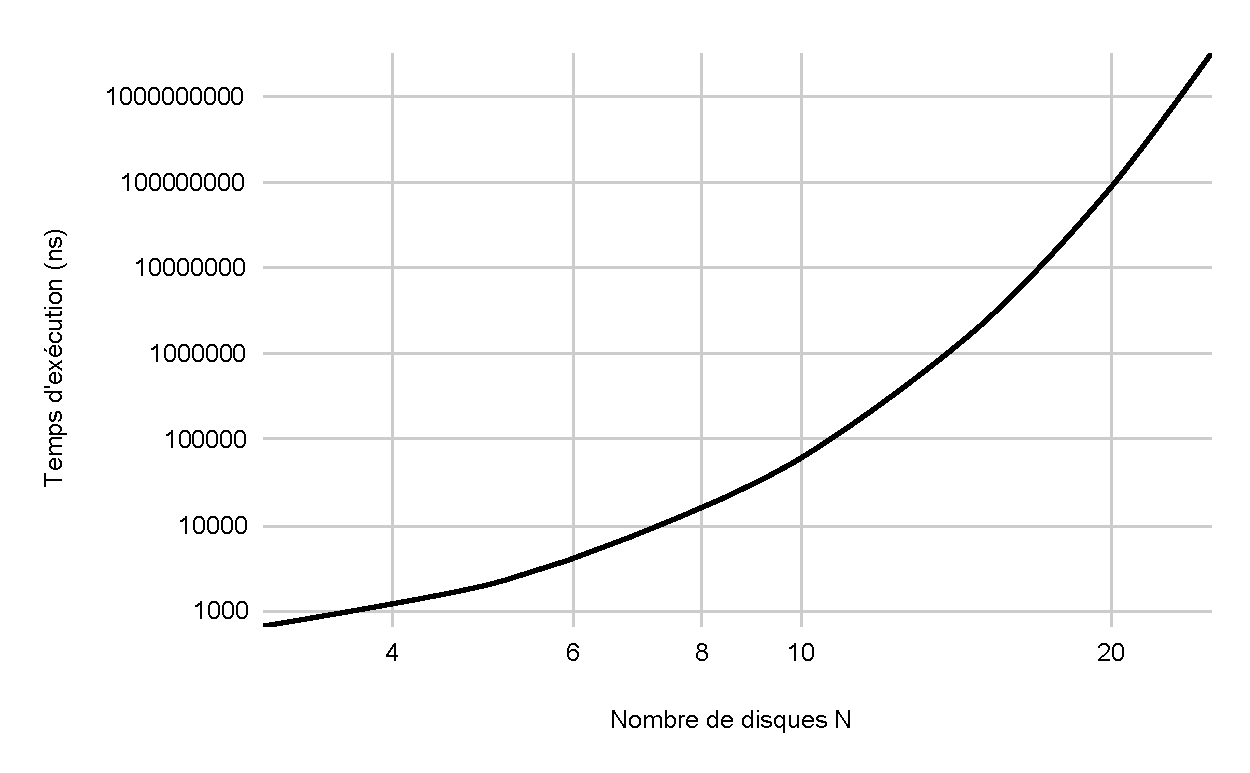
\includegraphics[scale=0.6]{./ressources/temps_execution_algo_reso.pdf}
        \caption{Temps d'exécution de l'algorithme de résolution}
    \label{fig:temps_exec_algo_reso}
\end{figure}
\par
Depuis la figure \ref{fig:temps_exec_algo_reso}, nous remarquons bien que le temps d'exécution de l'algorithme de résolution est exponentiel, conforme à la complexité de $\mathcal{O}(2^{n})$.

\subsection{Algorithme de génération de solution}
Cet algorithme fait au minimum $2^{n} - 1$ itérations, qui est équivalent au nombre d'étapes de la solution. Si l'algorithme génère à une étape un déplacement non autorisé, ce déplacement est rejeté et un autre est généré (si à son tour il n'est pas autorisé en génère un autre et ainsi de suite). Donc il est de complexité $\mathcal{O}(2^{n})$.
\par
Le tableau suivant représente les temps d'exécution en nanoseconde de l'algorithme de génération de solution pour le problème des tours de hanois selon la variation du nombre de disques.\\
\small
\begin{center}
    \begin{tabular}{| c | c | c | c | c | c | c | c |}
        \hline
        N & 3 & 5 & 7 & 10 & 15 & 20 & 25\\
        \hline
        t1(ns) & 16484 & 25099 & 73290 & 304737 & 11255800 & 401042000 & 14478900000\\
        \hline
        t2(ns) & 13480 & 23469 & 72592 & 310506 & 11503700 & 402620000 & 14470300000\\
        \hline
        t3(ns) & 15804 & 22381 & 70229 & 321948 & 11607800 & 401610000 & 14440400000\\
        \hline
        t4(ns) & 16334 & 24410 & 69875 & 312012 & 11348400 & 401075000 & 14418900000\\
        \hline
        t5(ns) & 15780 & 23887 & 79824 & 329052 & 11008400 & 402276000 & 14439500000\\
        \hline
        t6(ns) & 14275 & 21296 & 72074 & 321122 & 11444300 & 402046000 & 14443800000\\
        \hline
        t7(ns) & 13965 & 30082 & 52879 & 309217 & 1,17E+07 & 405221000 & 14440000000\\
        \hline
        t8(ns) & 14042 & 22535 & 62667 & 310238 & 1,14E+07 & 405030000 & 14471900000\\
        \hline
        t9(ns) & 13832 & 22679 & 49077 & 311514 & 11376700 & 405483000 & 14419800000\\
        \hline
        t10(ns) & 15764 & 22572 & 69374 & 311673 & 11215200 & 402717000 & 14449700000\\
        \hline
        moyenne(ns) & 14976 & 23841 & 67188 & 314202 & 11386730 & 402912000 & 14447320000\\
        \hline
    \end{tabular}
\end{center}
\normalsize
\par
La figure suivante (voir Figure \ref{fig:temps_exec_algo_generation}) représente l'évolution du temps d'exécution selon le nombre de disques.

\begin{figure}[H]
    \centering
        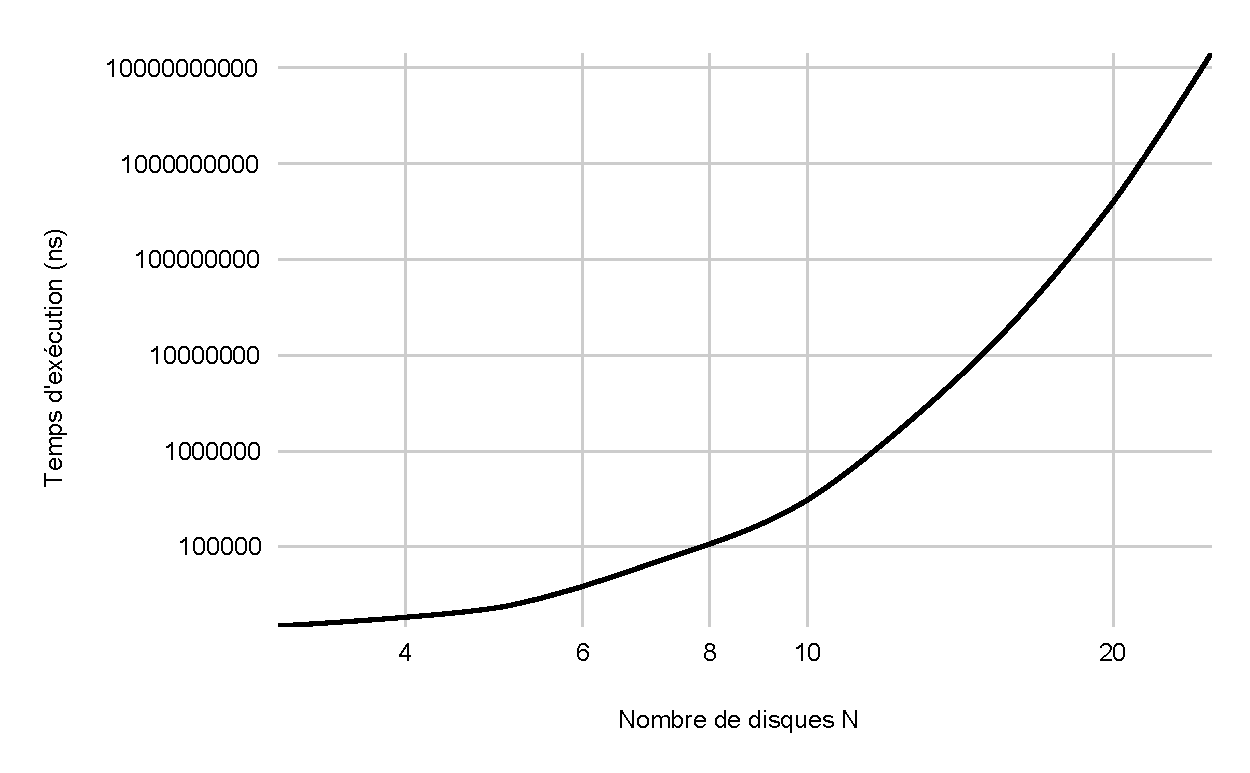
\includegraphics[scale=0.6]{./ressources/temps_execution_algo_generation.pdf}
        \caption{Temps d'exécution de l'algorithme de génération de solution}
    \label{fig:temps_exec_algo_generation}
\end{figure}
\par
Depuis la figure \ref{fig:temps_exec_algo_generation}, nous remarquons bien que le temps d'exécution de l'algorithme de résolution est exponentiel, conforme à la complexité de $\mathcal{O}(2^{n})$. Cependant, les temps d'exécution sont bien plus élevés que ceux de l'algorithme de résolution, car même si l'algorithme de génération fait $2^{n} - 1$ itération, certains déplacements sont rejetés.

\subsection{Algorithme de vérification de solution}
Le tableau suivant représente les temps d'exécution en nanoseconde de l'algorithme de vérification de solution pour le problème des tours de hanois selon la variation du nombre de disques.\\
\small
\begin{center}
    \begin{tabular}{| c | c | c | c | c | c | c | c |}
        \hline
        N & 3 & 5 & 7 & 10 & 15 & 20 & 25\\
        \hline
        t1(ns) & 71 & 61 & 113 & 80 & 75 & 146 & 182\\
        \hline
        t2(ns) & 61 & 68 & 111 & 68 & 77 & 94 & 61\\
        \hline
        t3(ns) & 66 & 95 & 66 & 80 & 143 & 84 & 156\\
        \hline
        t4(ns) & 68 & 68 & 82 & 66 & 101 & 86 & 143\\
        \hline
        t5(ns) & 76 & 75 & 97 & 108 & 65 & 141 & 197\\
        \hline
        t6(ns) & 57 & 67 & 81 & 110 & 64 & 104 & 179\\
        \hline
        t7(ns) & 58 & 90 & 77 & 104 & 180 & 148 & 91\\
        \hline
        t8(ns) & 74 & 73 & 70 & 78 & 137 & 147 & 102\\
        \hline
        t9(ns) & 78 & 75 & 74 & 117 & 105 & 126 & 105\\
        \hline
        t10(ns) & 60 & 66 & 68 & 80 & 68 & 78 & 164\\
        \hline
        moyenne(ns) & 67 & 74 & 84 & 89 & 102 & 115 & 138\\
        \hline
    \end{tabular}
\end{center}
\normalsize
\par
La figure suivante (voir Figure \ref{fig:temps_exec_algo_verification}) représente l'évolution du temps d'exécution selon le nombre de disques.

\begin{figure}[H]
    \centering
        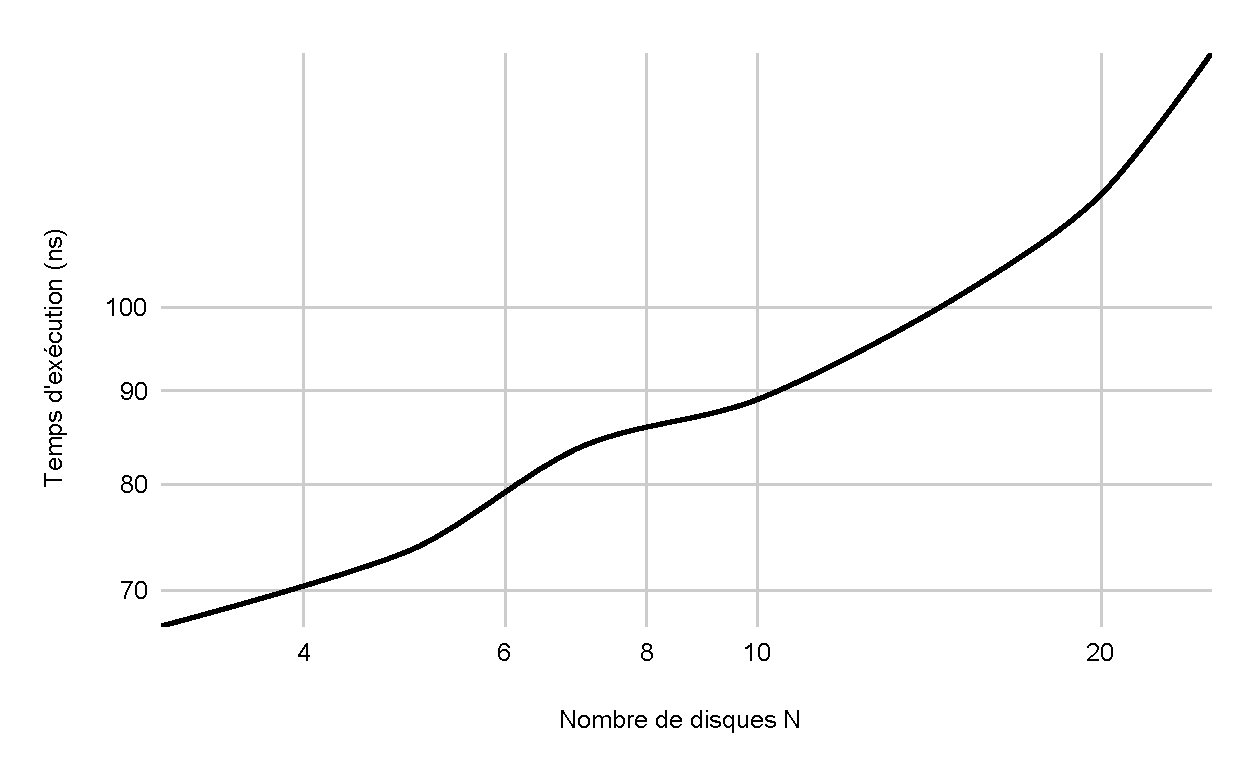
\includegraphics[scale=0.6]{./ressources/temps_execution_algo_verification.pdf}
        \caption{Temps d'exécution de l'algorithme de vérification de solution}
    \label{fig:temps_exec_algo_verification}
\end{figure}
\par
Depuis la figure \ref{fig:temps_exec_algo_verification}, nous observons une trajectoire presque linéaire, qui est représentative de la complexité $\mathcal{O}(n)$. Les fluctuations sont dûes au nombre de disques relativement bas.

\paragraph{Discussion des résultats}
On constate que la complexité de l'algorithme de résolution pour le problème des tours de hanoi évolue bien de manière exponentielle comme l'a montré l'étude expérimentale. Le temps d'exécution pour une instance du problème de 20 disques est de l'ordre de dizaine de secondes, celle avec 30 disques dépasse les quinzaines de minutes. Avec de tels résultats, il est clair que l'exploitation effective de ce genre de complexités est inenvisageable, voire impossible.
\par
Quant à l'algorithme de vérification, il a une simple complexité linéaire. Il ne fait que vérifier l'état de la dernière tour, les déplacements quant à eux, sont supposés corrects et valides par l'algorithme de génération de solution.


    \newpage
    \onehalfspacing
    \chapter{Conclusion générale}

\section{Conclusion}
Dans ce rapport, nous explorons comment le jeu d'enfant classique de la tour de Hanoï peut être utilisé à un niveau élaboré ou élémentaire. Il peut être exploité pour la vulgarisation des concepts mathématiques et pousse le joueur débutant à la réflexion en résolvant le jeu avec 3 ou 4 disques, tandis que les  plus avancés peuvent se poser plusieurs questions sur les liens de la structure avec les systèmes de numération, la modification des règles et d'autres questions qui sont encore l'objet des recherches d'aujourd'hui.\\
Nous avons commencé l'exploration en présentant le problème, son origine et sa définition formelle pour trouver la solution. \\
Dans le deuxième chapitre, nous avons entamer le processus de la résolution en modélisant cette dernière. Nous avons ensuite détaillé les algorithmes de solution et de vérification nécessaires ainsi que le calcul de leurs complexités. Finalement, nous avons illustrer une instance du problème avec la solution générée.  \\
Nous avons fini notre étude avec des expériences pour calculer les complexités théroriques (temporelle et spatiale) de nos algorithmes et les comparer aux résultats expérimentaux obtenus sur plusieurs essais.\\
L'expérimentation avec ce jeu offre à chacun l'occasion d'apprécier les ressorts du jeu, tels que ses aspects algorithmiques, les structures de données, les mathématiques appliquées, etc.\\
Par ailleurs, le jeu de la tour de Hanoï est un cas idéal pour illustrer la puissance
de la notion d’algorithme récursif et donne un exemple du calcul de factorielle $n$. En effet, son efficacité est impressionnante pour seulement quelques lignes de code. Contrairement à ce dernier type d'algorithme, un algorithme itératif de résolution de la tour de Hanoï est en général beaucoup moins facilement trouvé et est toujours plus long.

\end{document}
